%
% ---------------------------------------------------------------
% Copyright (C) 2012-2018 Gang Li
% ---------------------------------------------------------------
%
% This work is the default powerdot-tuliplab style test file and may be
% distributed and/or modified under the conditions of the LaTeX Project Public
% License, either version 1.3 of this license or (at your option) any later
% version. The latest version of this license is in
% http://www.latex-project.org/lppl.txt and version 1.3 or later is part of all
% distributions of LaTeX version 2003/12/01 or later.
%
% This work has the LPPL maintenance status "maintained".
%
% This Current Maintainer of this work is Gang Li.
%
%

\documentclass[
size=14pt,
paper=smartboard,  %a4paper, smartboard, screen
mode=present, 		%present, handout, print
display=slides, 	% slidesnotes, notes, slides
style=tuliplab,  	% TULIP Lab style
pauseslide,
fleqn,leqno]{powerdot}


\usepackage{cancel}
\usepackage{caption}
\usepackage{stackengine}
\usepackage{smartdiagram}
\usepackage{attrib}
\usepackage{amssymb}
\usepackage{amsmath} 
\usepackage{amsthm} 
\usepackage{mathtools}
\usepackage{rotating}
\usepackage{graphicx}
\usepackage{boxedminipage}
\usepackage{rotate}
\usepackage{calc}
\usepackage[absolute]{textpos}
\usepackage{psfrag,overpic}
\usepackage{fouriernc}
\usepackage{pstricks,pst-3d,pst-grad,pstricks-add,pst-text,pst-node,pst-tree}
\usepackage{moreverb,epsfig,subfigure}
\usepackage{color}
\usepackage{booktabs}
\usepackage{etex}
\usepackage{breqn}
\usepackage{multirow}
\usepackage{natbib}
\usepackage{bibentry}
\usepackage{gitinfo2}
\usepackage{siunitx}
\usepackage{nicefrac}
%\usepackage{geometry}
%\geometry{verbose,letterpaper}
\usepackage{media9}
\usepackage{animate}
%\usepackage{movie15}
\usepackage{auto-pst-pdf}

\usepackage{breakurl}
\usepackage{fontawesome}
\usepackage{xcolor}
\usepackage{multicol}



\usepackage{verbatim}
\usepackage[utf8]{inputenc}
\usepackage{dtk-logos}
\usepackage{tikz}
\usepackage{adigraph}
%\usepackage{tkz-graph}
\usepackage{hyperref}
%\usepackage{ulem}
\usepackage{pgfplots}
\usepackage{verbatim}
\usepackage{fontawesome} 


\usepackage{todonotes}
% \usepackage{pst-rel-points}
\usepackage{animate}
\usepackage{fontawesome}
\usepackage{graphicx}
\usepackage{listings}
\lstset{frameround=fttt,
	frame=trBL,
	stringstyle=\ttfamily,
	backgroundcolor=\color{yellow!20},
	basicstyle=\footnotesize\ttfamily}
\lstnewenvironment{code}{
	\lstset{frame=single,escapeinside=`',
		backgroundcolor=\color{yellow!20},
		basicstyle=\footnotesize\ttfamily}
}{}


\usepackage{hyperref}

\hypersetup{ % TODO: PDF meta Data
	pdftitle={Presentation Title},
	pdfauthor={Yao Yang},
	pdfpagemode={FullScreen},
	pdfborder={0 0 0}
}


% \usepackage{auto-pst-pdf}
% package to show source code

\definecolor{LightGray}{rgb}{0.9,0.9,0.9}
\newlength{\pixel}\setlength\pixel{0.000714285714\slidewidth}
\setlength{\TPHorizModule}{\slidewidth}
\setlength{\TPVertModule}{\slideheight}
\newcommand\highlight[1]{\fbox{#1}}
\newcommand\icite[1]{{\footnotesize [#1]}}

\newcommand\twotonebox[2]{\fcolorbox{pdcolor2}{pdcolor2}
	{#1\vphantom{#2}}\fcolorbox{pdcolor2}{white}{#2\vphantom{#1}}}
\newcommand\twotoneboxo[2]{\fcolorbox{pdcolor2}{pdcolor2}
	{#1}\fcolorbox{pdcolor2}{white}{#2}}
\newcommand\vpspace[1]{\vphantom{\vspace{#1}}}
\newcommand\hpspace[1]{\hphantom{\hspace{#1}}}
\newcommand\COMMENT[1]{}

\newcommand\placepos[3]{\hbox to\z@{\kern#1
		\raisebox{-#2}[\z@][\z@]{#3}\hss}\ignorespaces}

\renewcommand{\baselinestretch}{1.2}


\newcommand{\draftnote}[3]{
	\todo[author=#2,color=#1!30,size=\footnotesize]{\textsf{#3}}	}
% TODO: add yourself here:
%
\newcommand{\gangli}[1]{\draftnote{blue}{GLi:}{#1}}
\newcommand{\shaoni}[1]{\draftnote{green}{sn:}{#1}}
\newcommand{\gliMarker}
{\todo[author=GLi,size=\tiny,inline,color=blue!40]
	{Gang Li has worked up to here.}}
\newcommand{\snMarker}
{\todo[author=Sn,size=\tiny,inline,color=green!40]
	{Shaoni has worked up to here.}}

%%%%%%%%%%%%%%%%%%%%%%%%%%%%%%%%%%%%%%%%%%%%%%%%%%%%%%%%%%%%%%%%%%%%%%%%
% title
% TODO: Customize to your Own Title, Name, Address
%
\title{Bike Sharing Demand}
\author{
	YAO YANG
	\\
	\\Chongqing University of Posts and Telecommunications test
}
\date{\today}


% Customize the setting of slides
\pdsetup{
	% TODO: Customize the left footer, and right footer
	rf=\href{http://www.tulip.org.au}{
		Last Changed by: \textsc{\gitCommitterName}\ \gitVtagn-\gitAbbrevHash\ (\gitAuthorDate)
	},
	cf={Group Outlying Aspects Mining},
}


\begin{document}
	
	\maketitle
	
	%\begin{slide}{Overview}
	%\tableofcontents[content=sections]
	%\end{slide}
	
	
	%%==========================================================================================
	%%
	\begin{slide}[toc=,bm=]{Overview}
		\tableofcontents[content=currentsection,type=1]
	\end{slide}
	%%
	%%==========================================================================================
	
	
	\section{Problem Definition}
	
	
	%%==========================================================================================
	%%
	\begin{slide}{Bike Sharing Demand}
		
		\begin{center}
			\twotonebox{\rotatebox{90}{Defn}}{\parbox{.86\textwidth}
				{The goal of this project is to forecast bike rental demand given the input feature like the duration of travel, departure location, arrival location, and time elapsed.}}
			\twotonebox{\rotatebox{90}{Defn}}{\parbox{.86\textwidth}
				{Evaluation metrics: RMSLE(Root Mean Squard Logarithmic Error) is required to evaluate the model.
					\\\\
					$ RMSLE =  \sqrt{\tfrac{1}{n}\sum_{i=1}^n\left[log(p_i+1)-log(a_i+1) \right]^2} $
					\\n is the number of test set samples, pi is the test value, and ai is the actual value. When the root mean square error is smaller, it means that the fitting effect of the data is better and the test value is closer to the actual value.
				}
			}
		\end{center}
		%%==========================================================================================
	\end{slide}
	%%==========================================================================================
	
	
	
	\section{Data Clean}
	%%==========================================================================================
	%%
	\begin{slide}{Data Describe}
		\begin{center}
			\twotonebox{\rotatebox{90}{Defn}}{\parbox{.86\textwidth}
				{You are provided hourly rental data spanning two years. For this competition, the training set is comprised of the first 19 days of each month, while the test set is the 20th to the end of the month. You must predict the total count of bikes rented during each hour111covered by the test set, using only information available prior to the rental period.
					\begin{itemize}
						\item \textcolor{orange}{train.csv} It contains a training set of target variables.
						\item \textcolor{orange}{test.csv} It does not contain a training set of target variables.
						\item \textcolor{orange}{sampleSubmission.csv} It is a properly formatted sample submission file.
					\end{itemize}
			}}
		\end{center}
	\end{slide}
	%%==========================================================================================
	
	\begin{slide}[toc=,bm=]{Data Describe}
		
		\begin{itemize}
			\item \textcolor{orange}{datetime} - hourly date + timestamp
			\item \textcolor{orange}{season} - 1 = spring, 2 = summer, 3 = fall, 4 = winter 
			\item \textcolor{orange}{holiday} - whether the day is considered a holiday
			\item \textcolor{orange}{workingday}  - whether the day is neither a weekend nor holiday
			\item \textcolor{orange}{weather} - 1: Clear, Few clouds, Partly cloudy, Partly cloudy
			\\2: Mist + Cloudy, Mist + Broken clouds, Mist + Few clouds, Mist
			\\3: Light Snow, Light Rain + Thunderstorm + Scattered clouds, Light Rain + Scattered clouds
			\\4: Heavy Rain + Ice Pallets + Thunderstorm + Mist, Snow + Fog
			\item \textcolor{orange}{temp} - temperature in Celsius
			\item \textcolor{orange}{atemp} - "feels like" temperature in Celsius
			\item \textcolor{orange}{humidity} - relative humidity
			\item \textcolor{orange}{windspeed} - wind speed
			\item \textcolor{orange}{casual} - number of non-registered user rentals initiated
			\item \textcolor{orange}{registered} - number of registered user rentals initiated
			\item \textcolor{orange}{count} - number of total rentals
		\end{itemize}
		
	\end{slide}
	%%==========================================================================================
	%%==========================================================================================
	%%
	\begin{slide}[toc=,bm=]{Data Describe}
		\begin{figure}
			\centering
			\selectcolormodel{rgb}
			\includegraphics[width=0.8\textwidth,height=0.5\textwidth]{variable.eps}
			\caption{Describe} \label{framework}
		\end{figure}
	\end{slide}
	%%==========================================================================================
	
	%%==========================================================================================
	%%
	\begin{slide}{Data Visualization Plot}
		\begin{figure}
			\centering
			\selectcolormodel{rgb}
			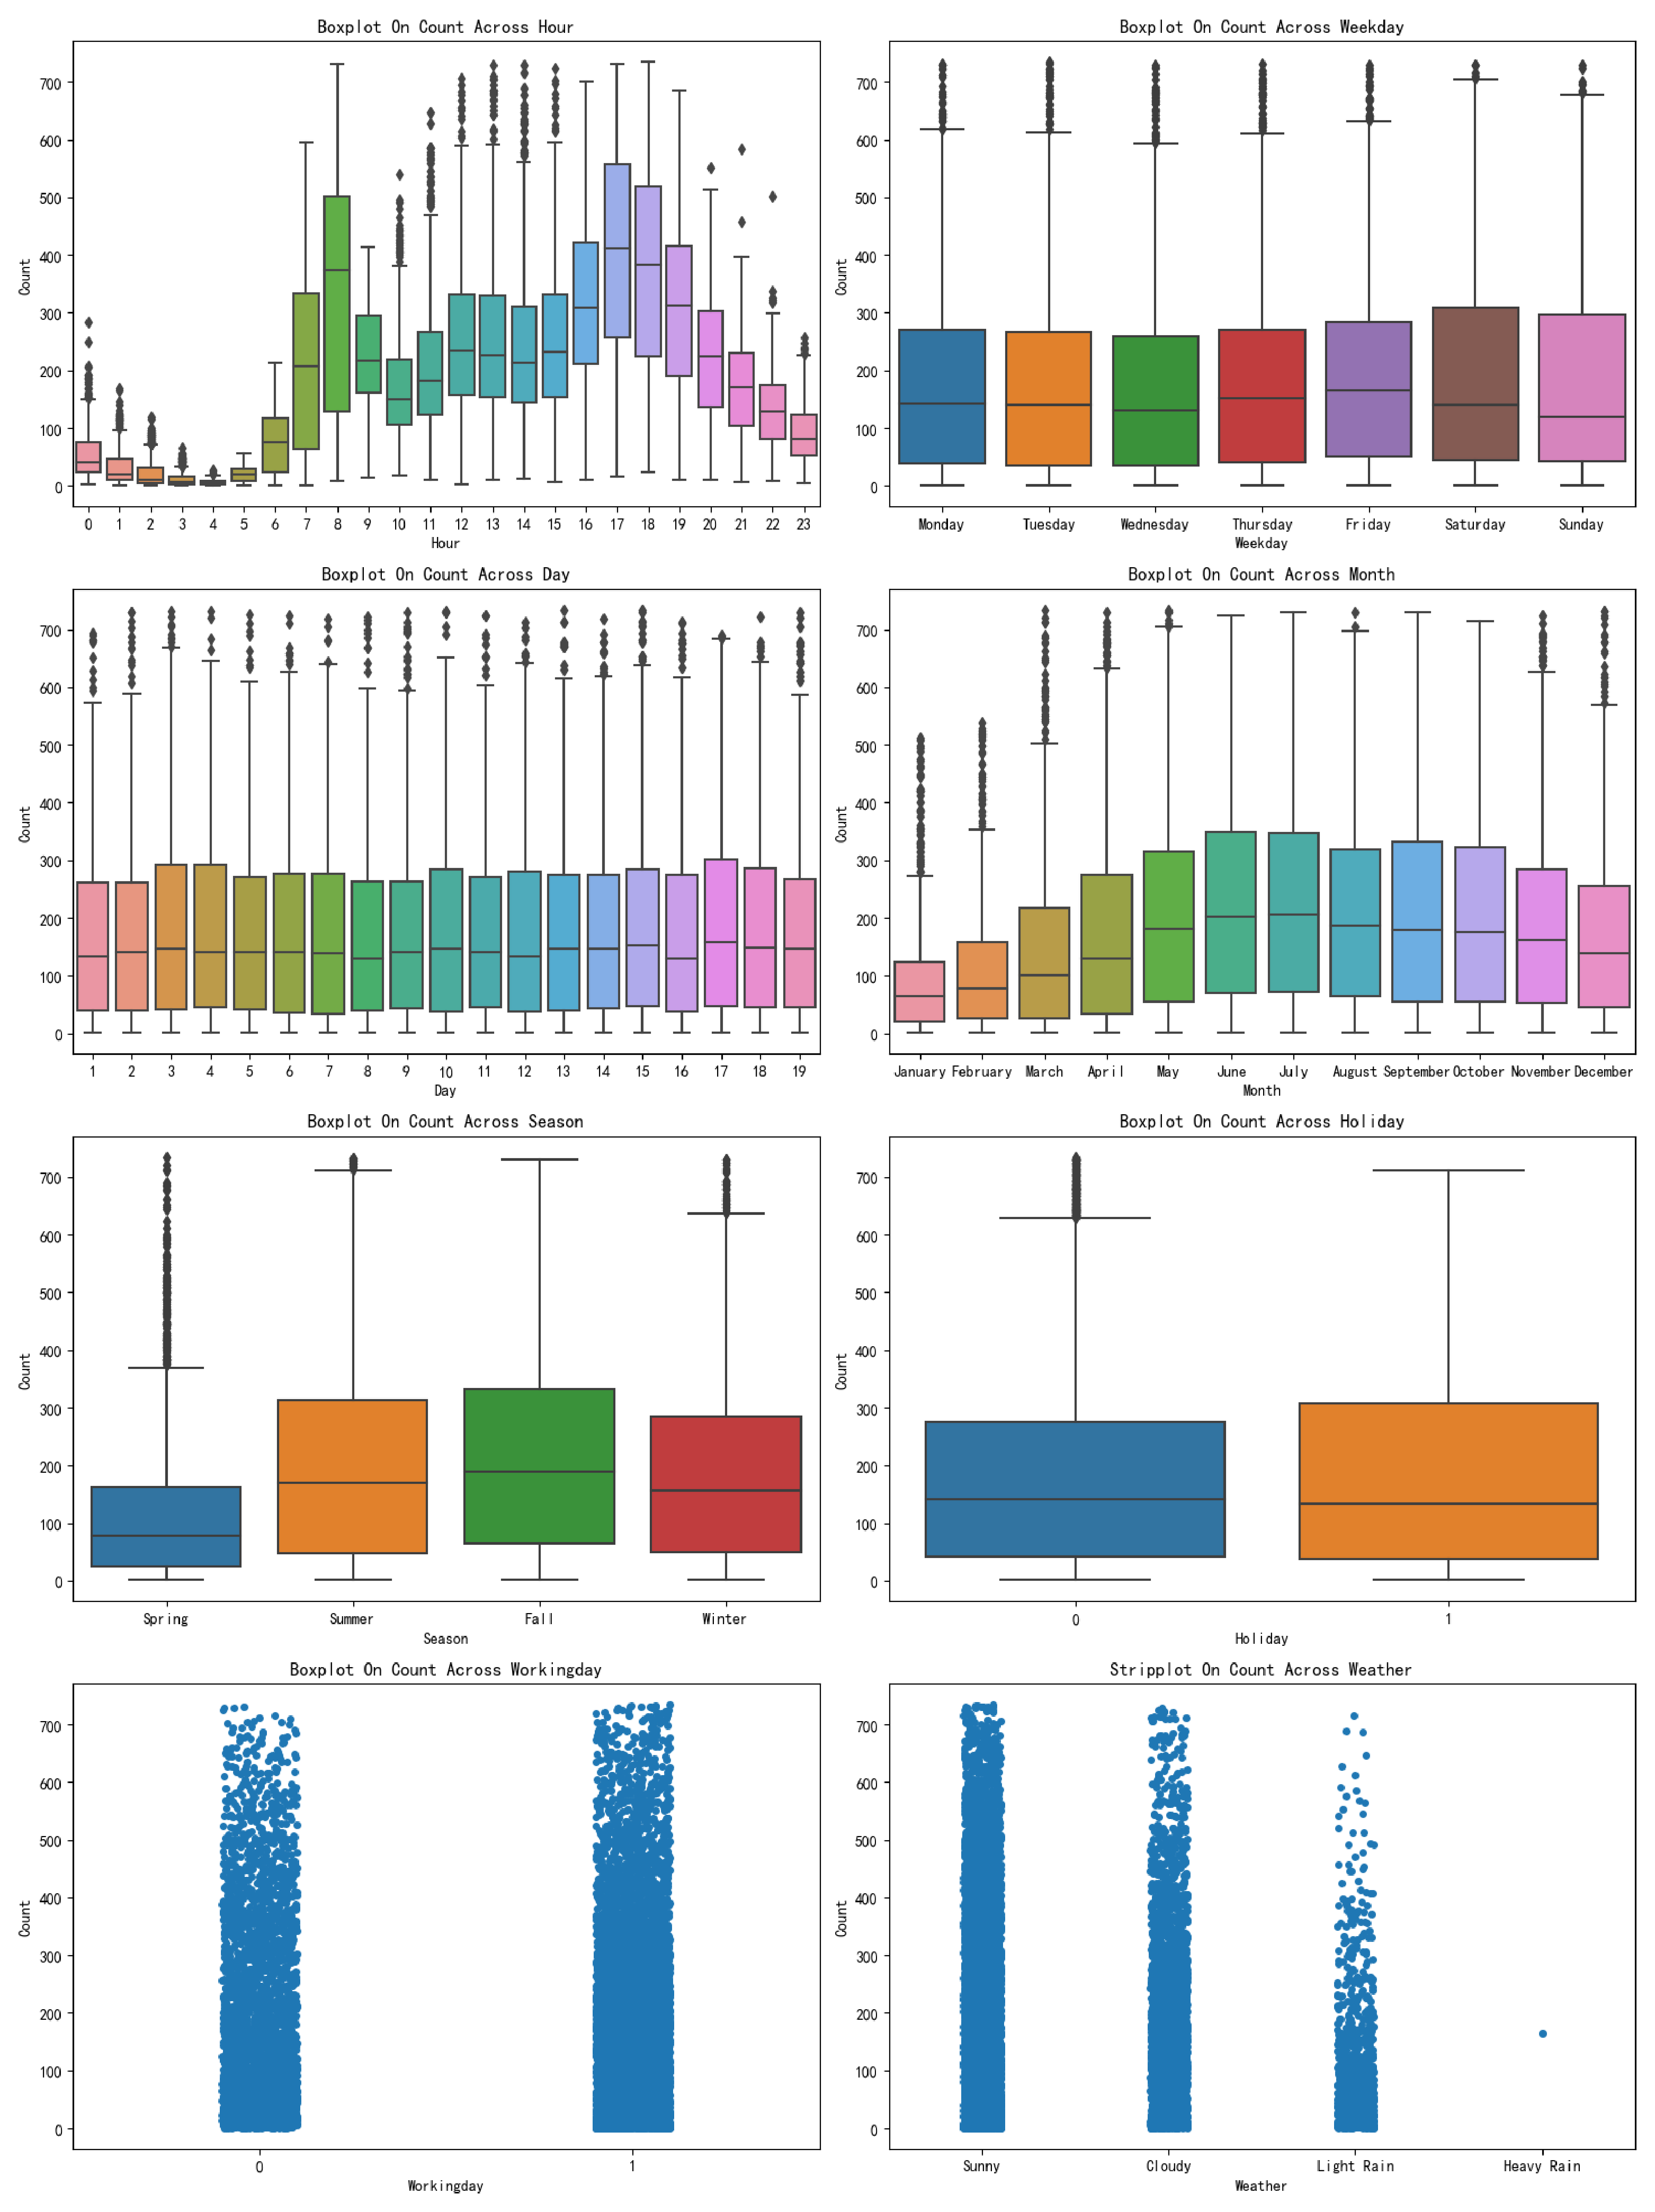
\includegraphics[width=0.8\textwidth,height=0.5\textwidth]{plot.eps}
			\caption{Box Plot and Scatter Plot} \label{framework}
		\end{figure}
	\end{slide}
	%%==========================================================================================
	
	%%==========================================================================================
	%%
	\begin{slide}[toc=,bm=]{Data Visualization Plot}
		\begin{figure}
			\centering
			\selectcolormodel{rgb}
			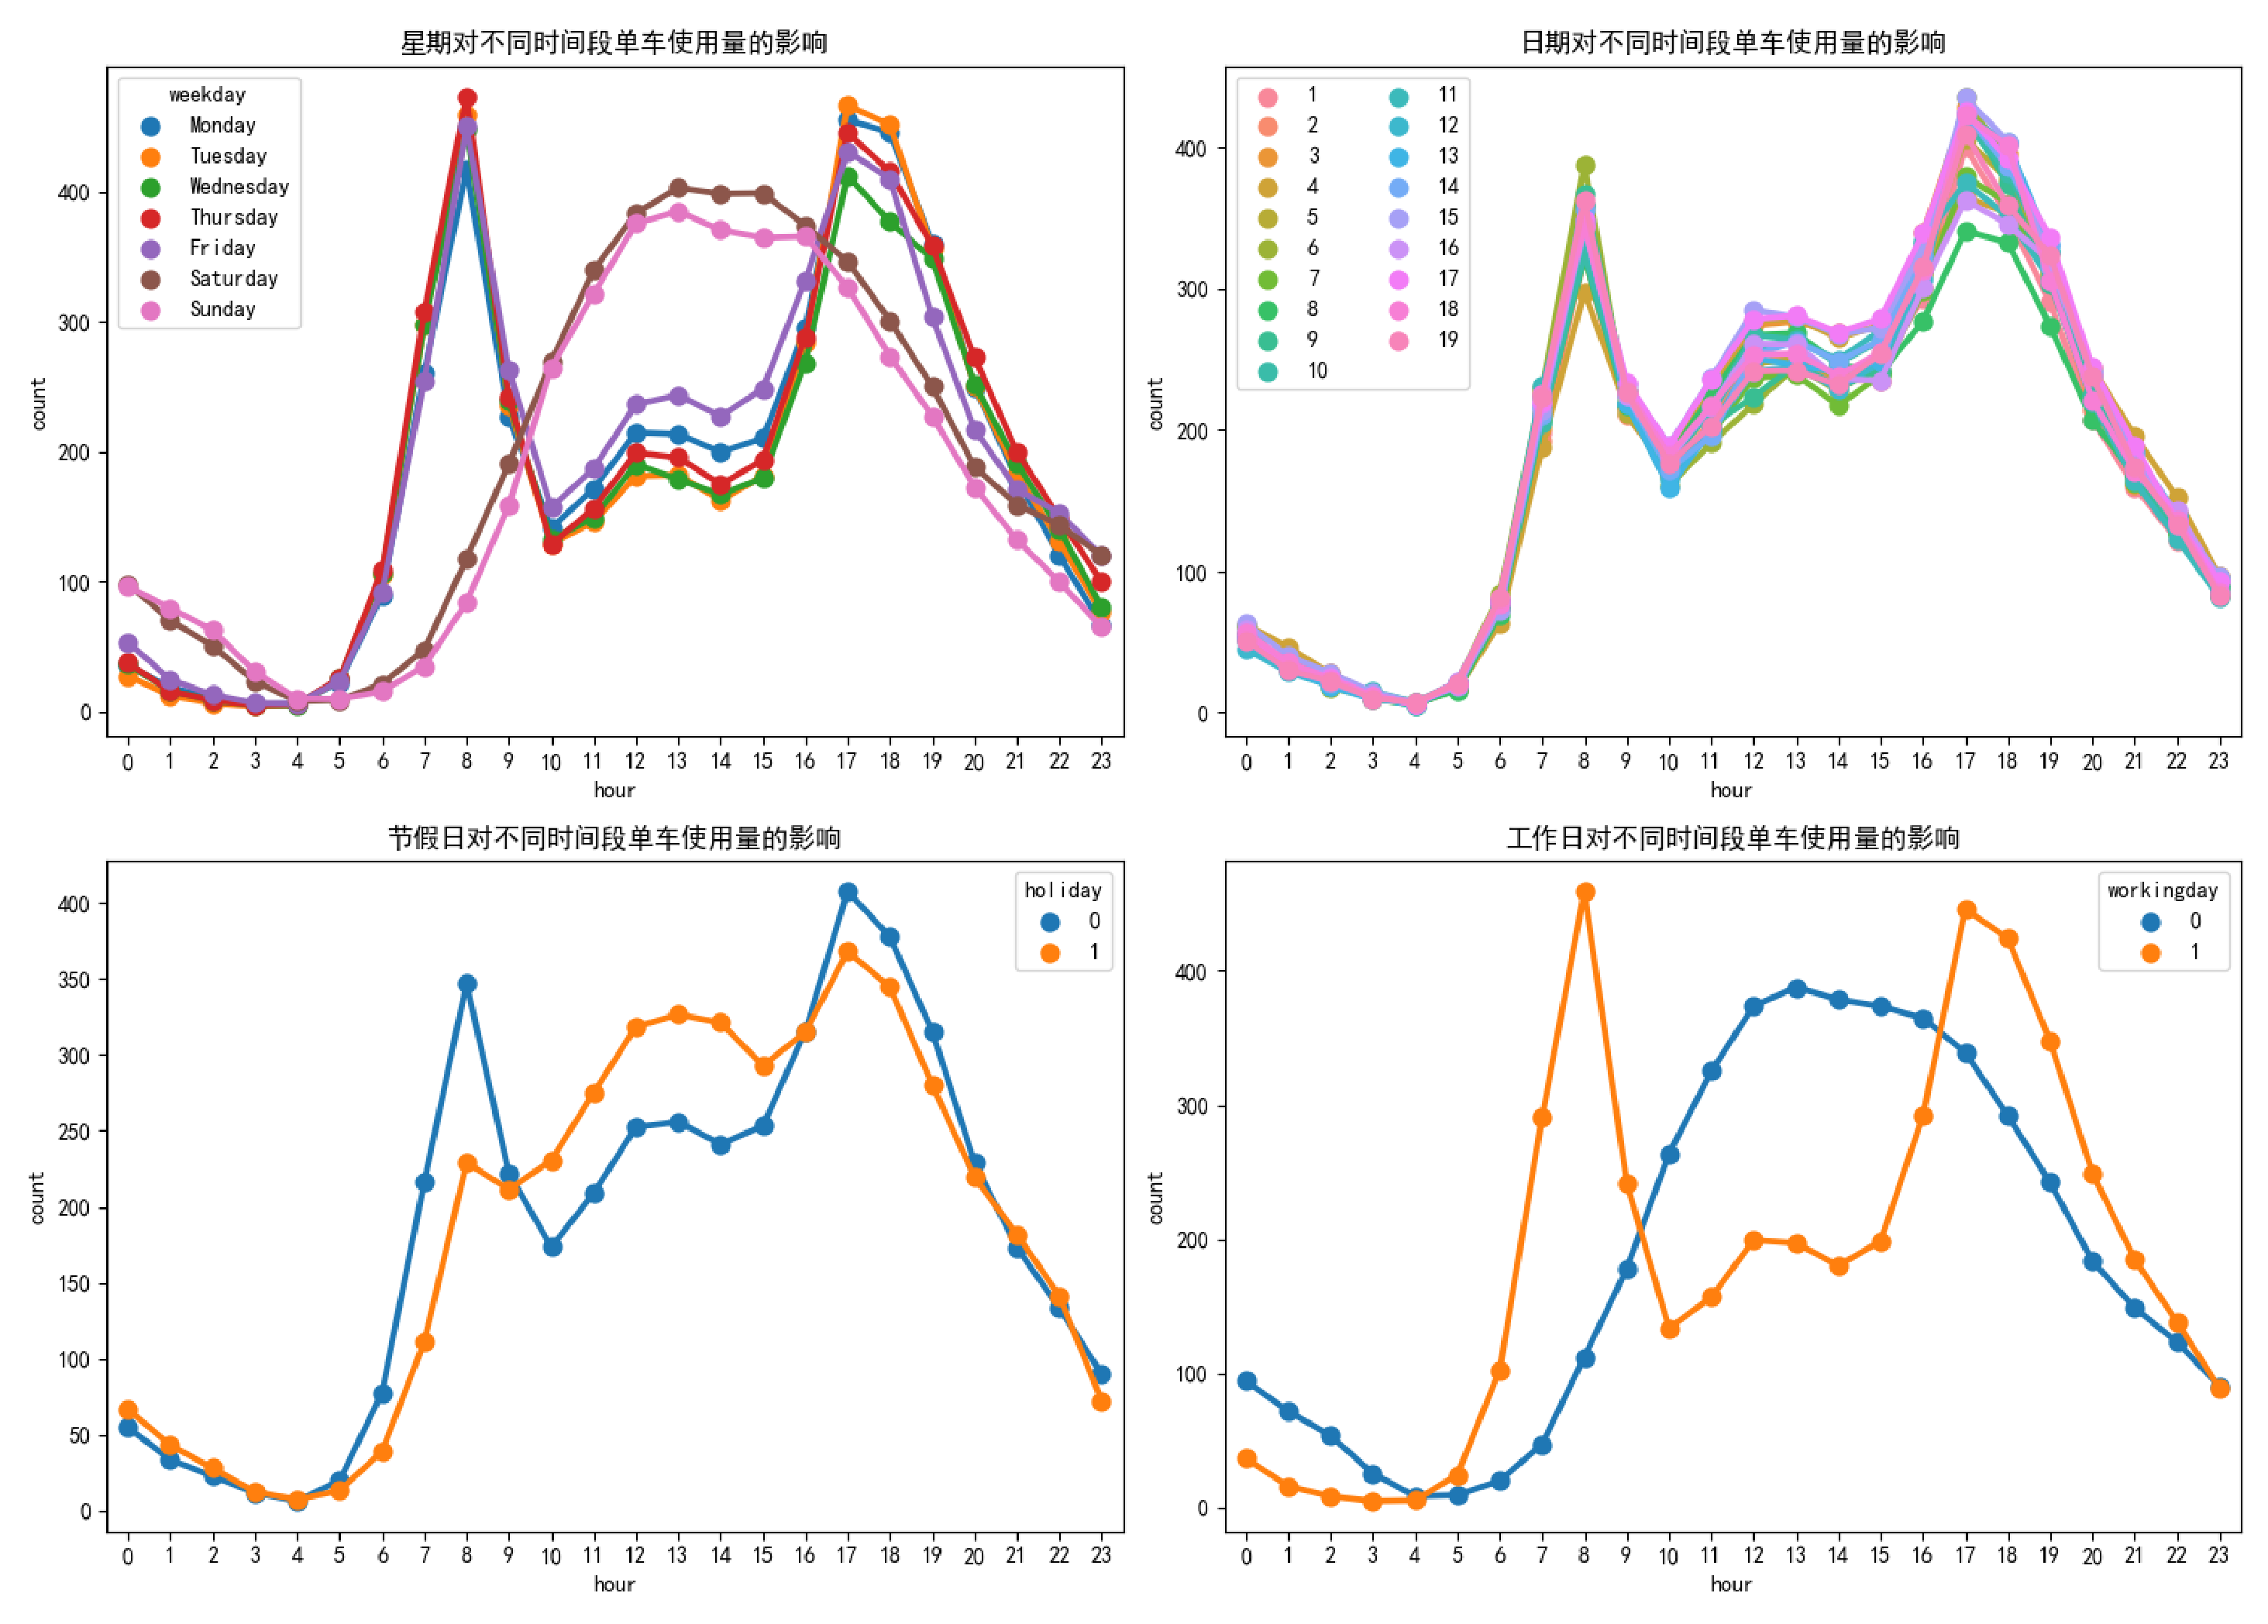
\includegraphics[width=0.8\textwidth,height=0.5\textwidth]{influence.eps}
			\caption{Line Chart} \label{framework}
		\end{figure}
	\end{slide}
	%%==========================================================================================
	
	%%==========================================================================================
	%% 
	\begin{slide}[toc=,bm=]{Data Visualization Plot}
		\begin{figure}
			\centering
			\selectcolormodel{rgb}
			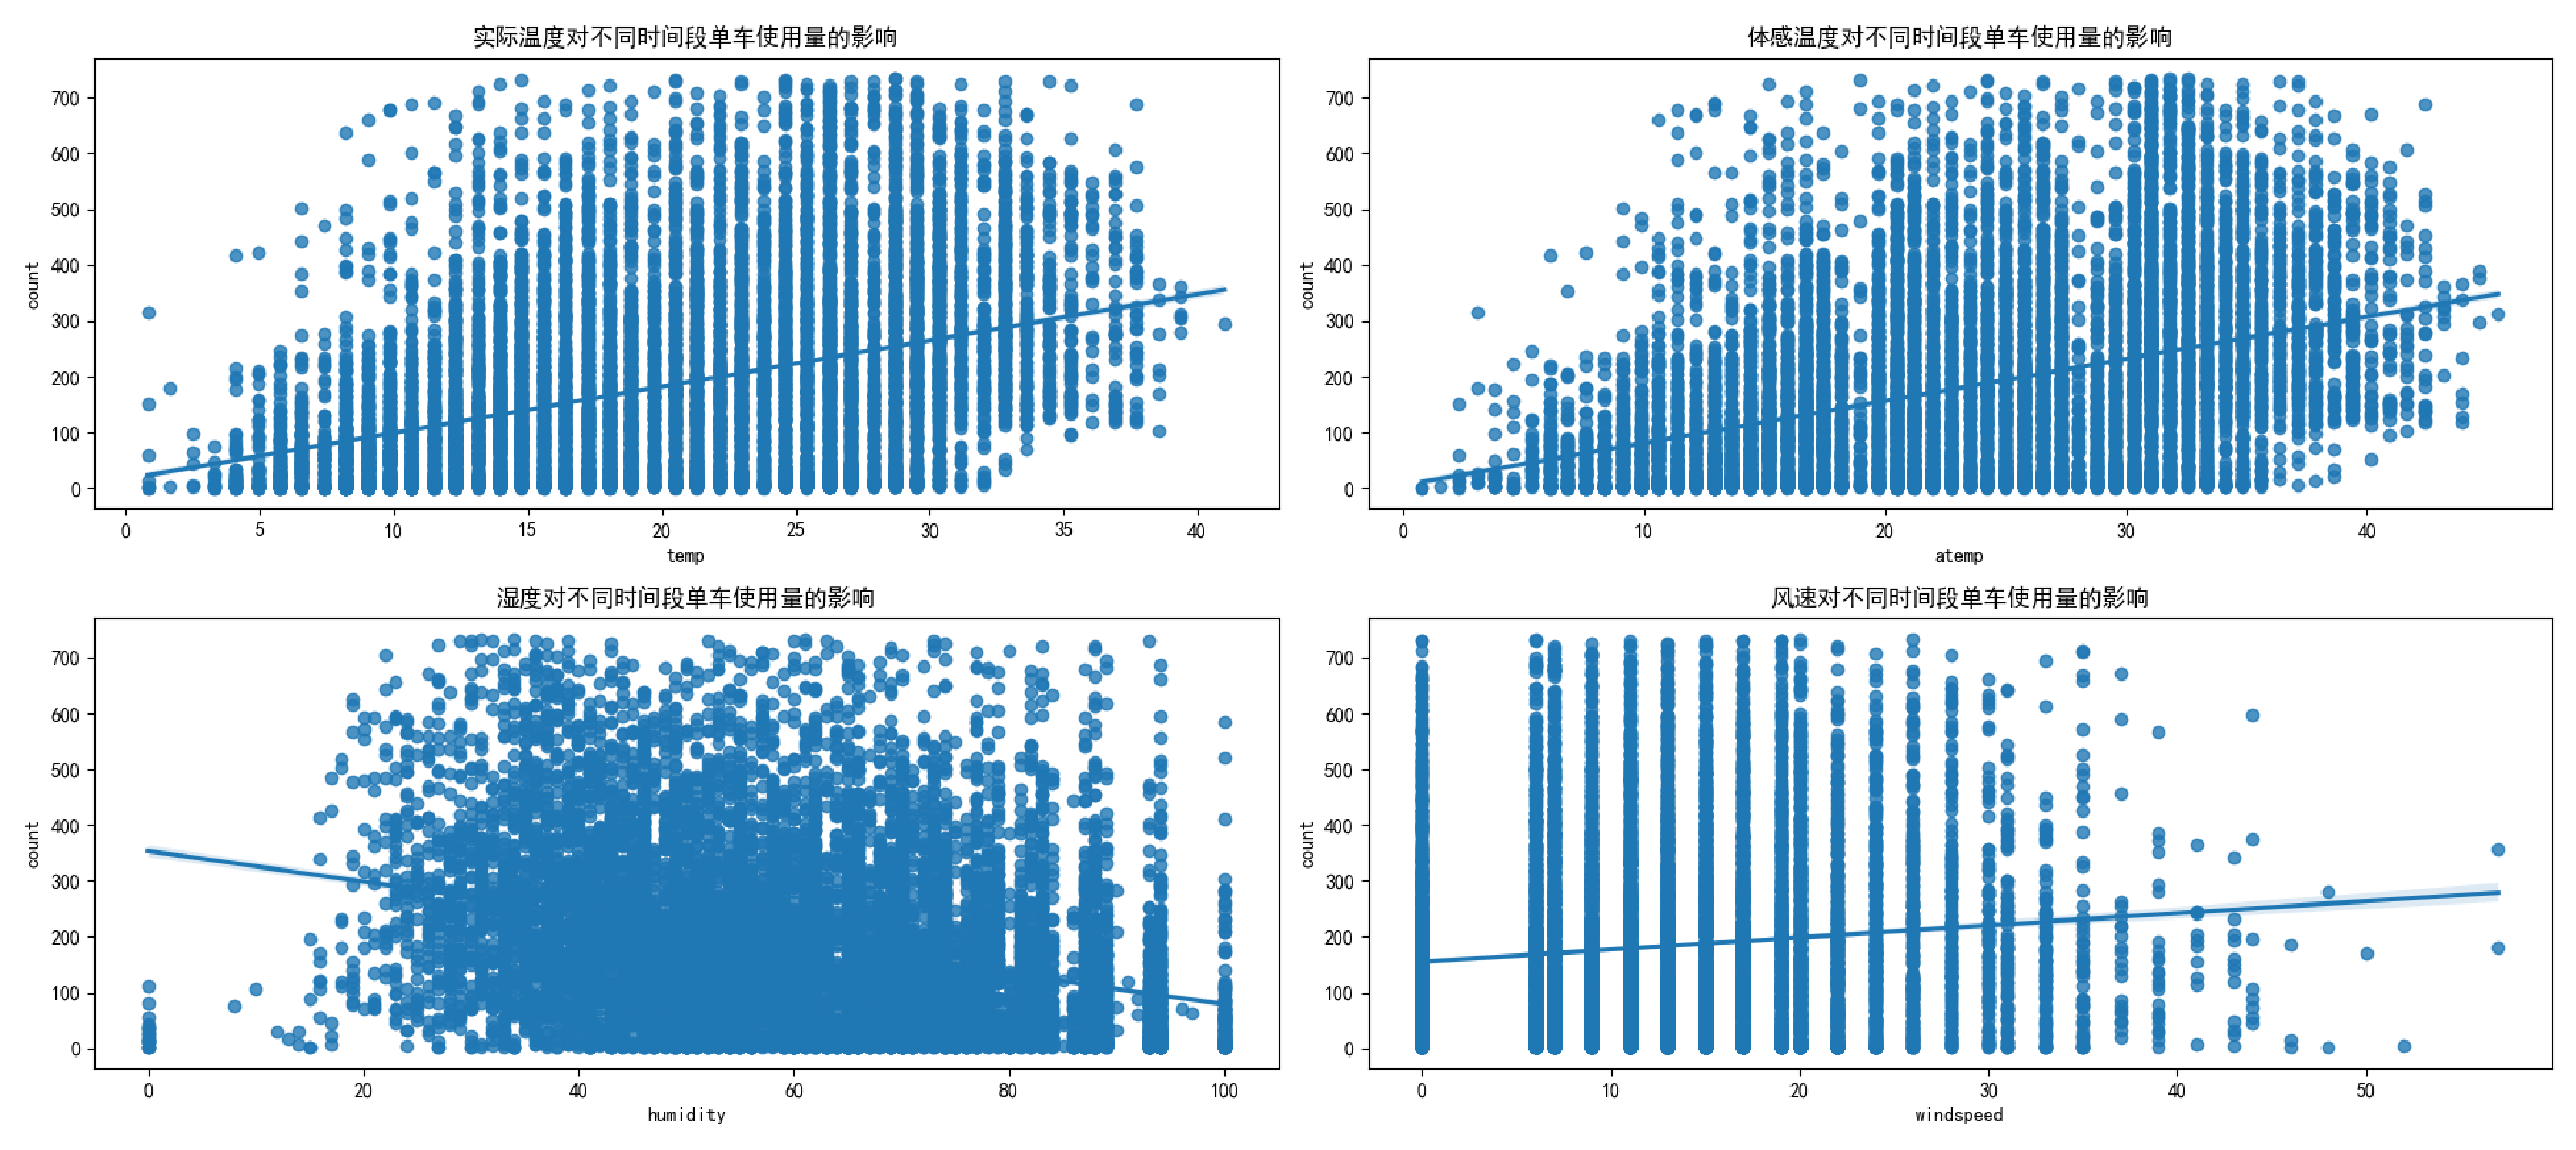
\includegraphics[width=0.8\textwidth,height=0.5\textwidth]{output.eps}
			\caption{Scatter Plot} \label{framework}
		\end{figure}
	\end{slide}
	%%==========================================================================================
	
	%%==========================================================================================
	%%
	\begin{slide}[toc=,bm=]{Data Visualization Plot}
		\begin{figure}
			\begin{center}
				\selectcolormodel{rgb}
				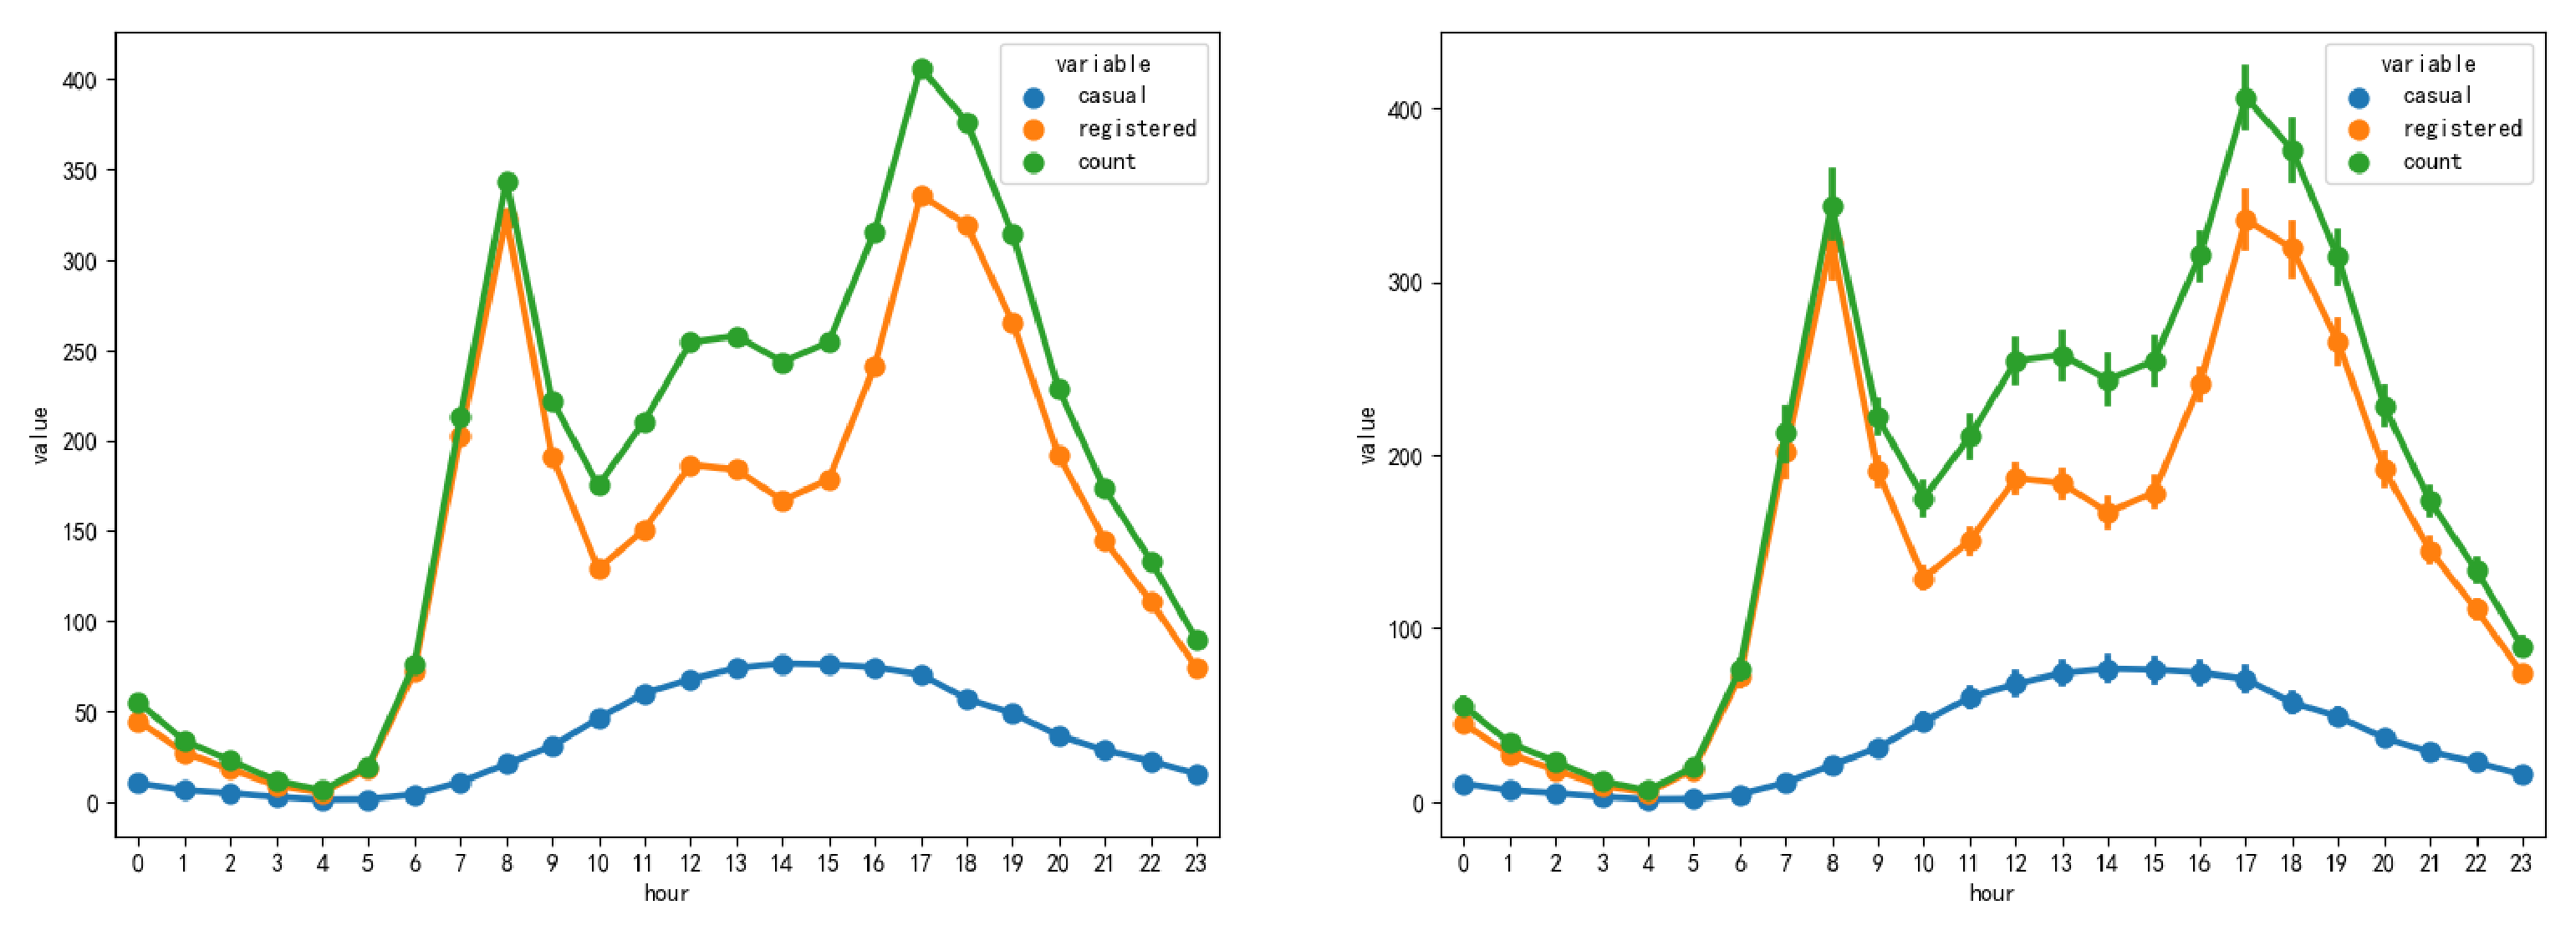
\includegraphics[width=0.8\textwidth]{user.eps}
				\caption{Line Chart} \label{framework}
			\end{center}
		\end{figure}
	\end{slide}
	%%==========================================================================================
	
	
	\section{Knowledge Discovery}
	%%==========================================================================================
	%%
	\begin{slide}{Variable Relationship Discovery}
		\begin{figure}
			\centering
			\selectcolormodel{rgb}
			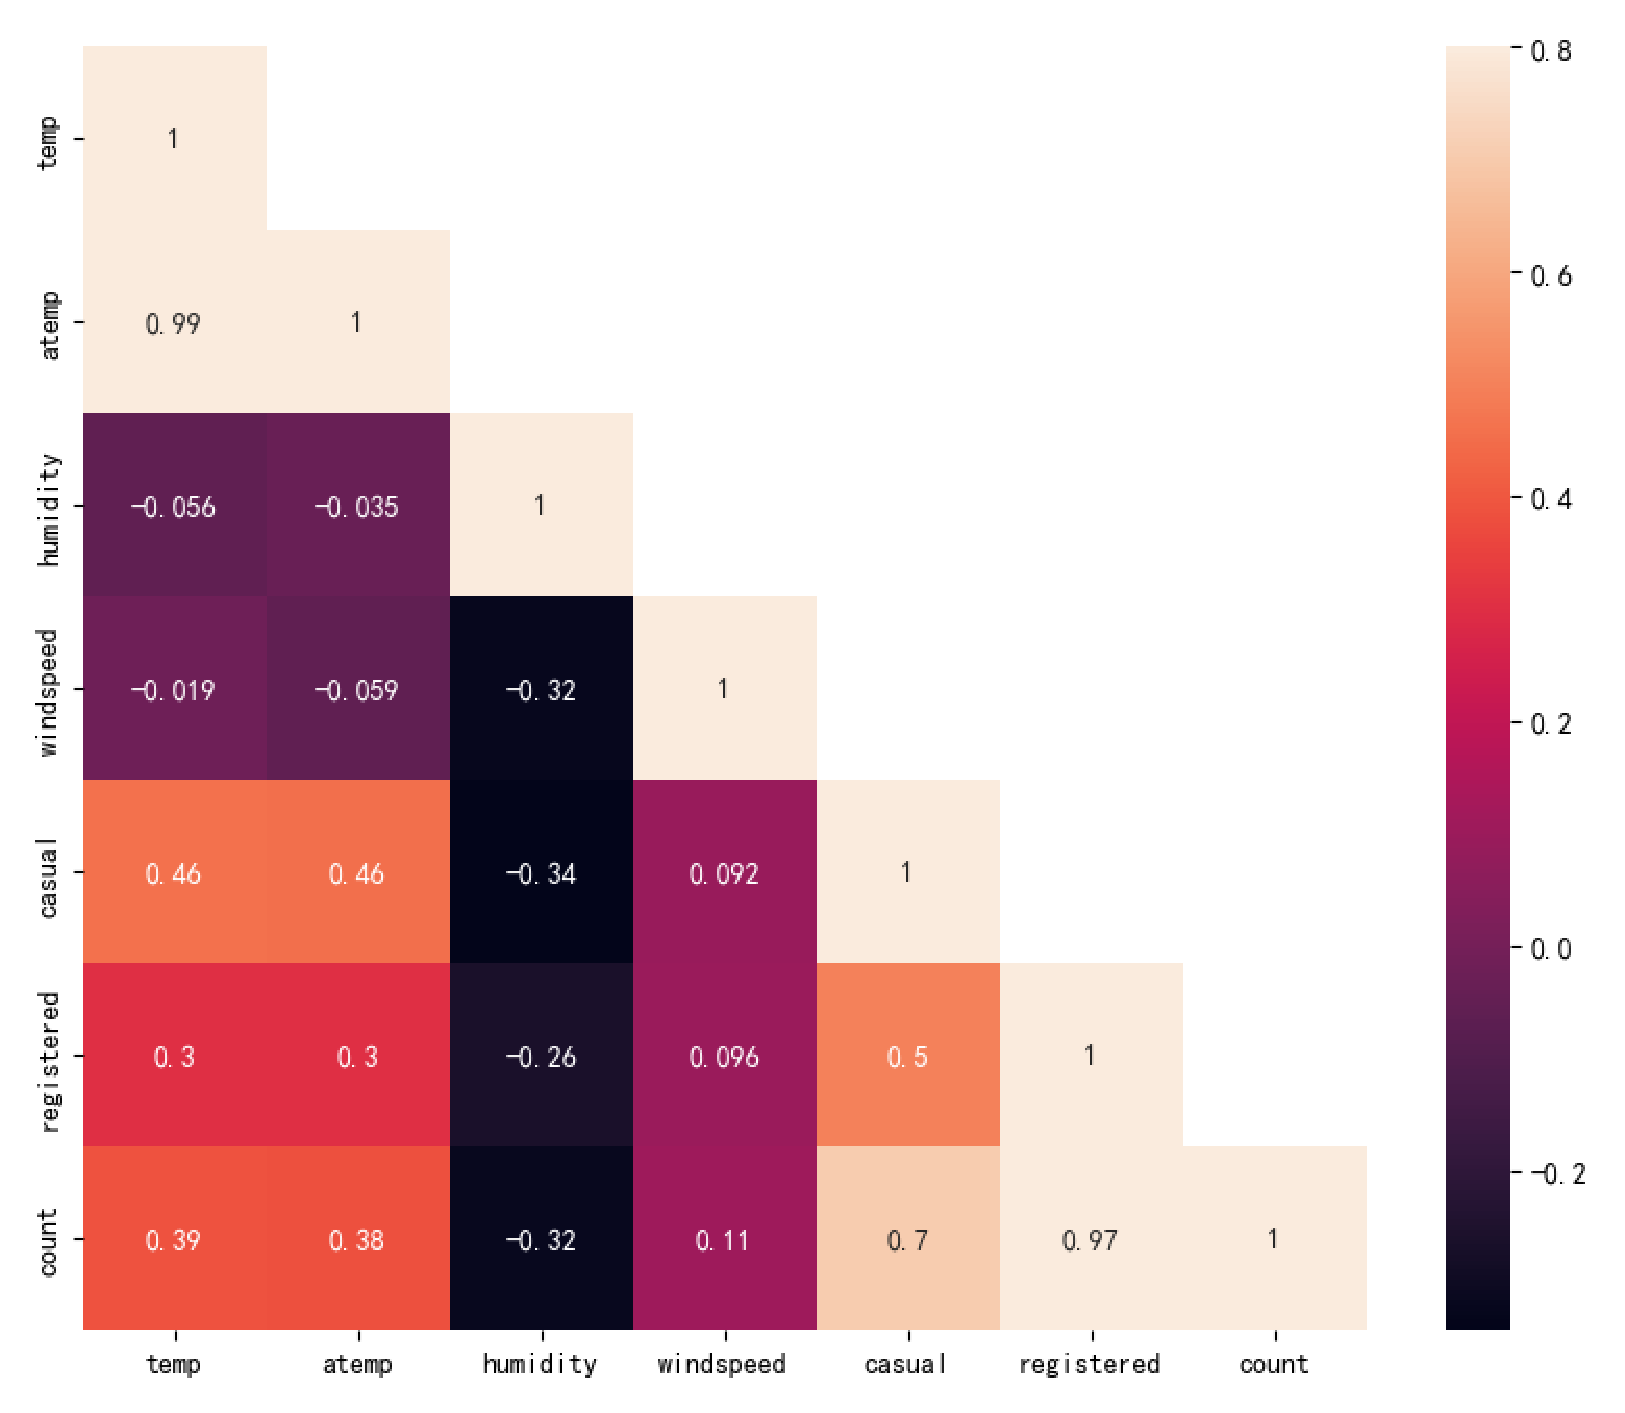
\includegraphics[width=0.8\textwidth,height=0.5\textwidth]{juzhen.eps}
			\caption{Hot Map} \label{framework}
		\end{figure}
	\end{slide}
	%%==========================================================================================
	
	%%==========================================================================================
	%%
	
	\begin{slide}{Target Variable Analysis}
		\begin{figure}
			\centering
			\selectcolormodel{rgb}
			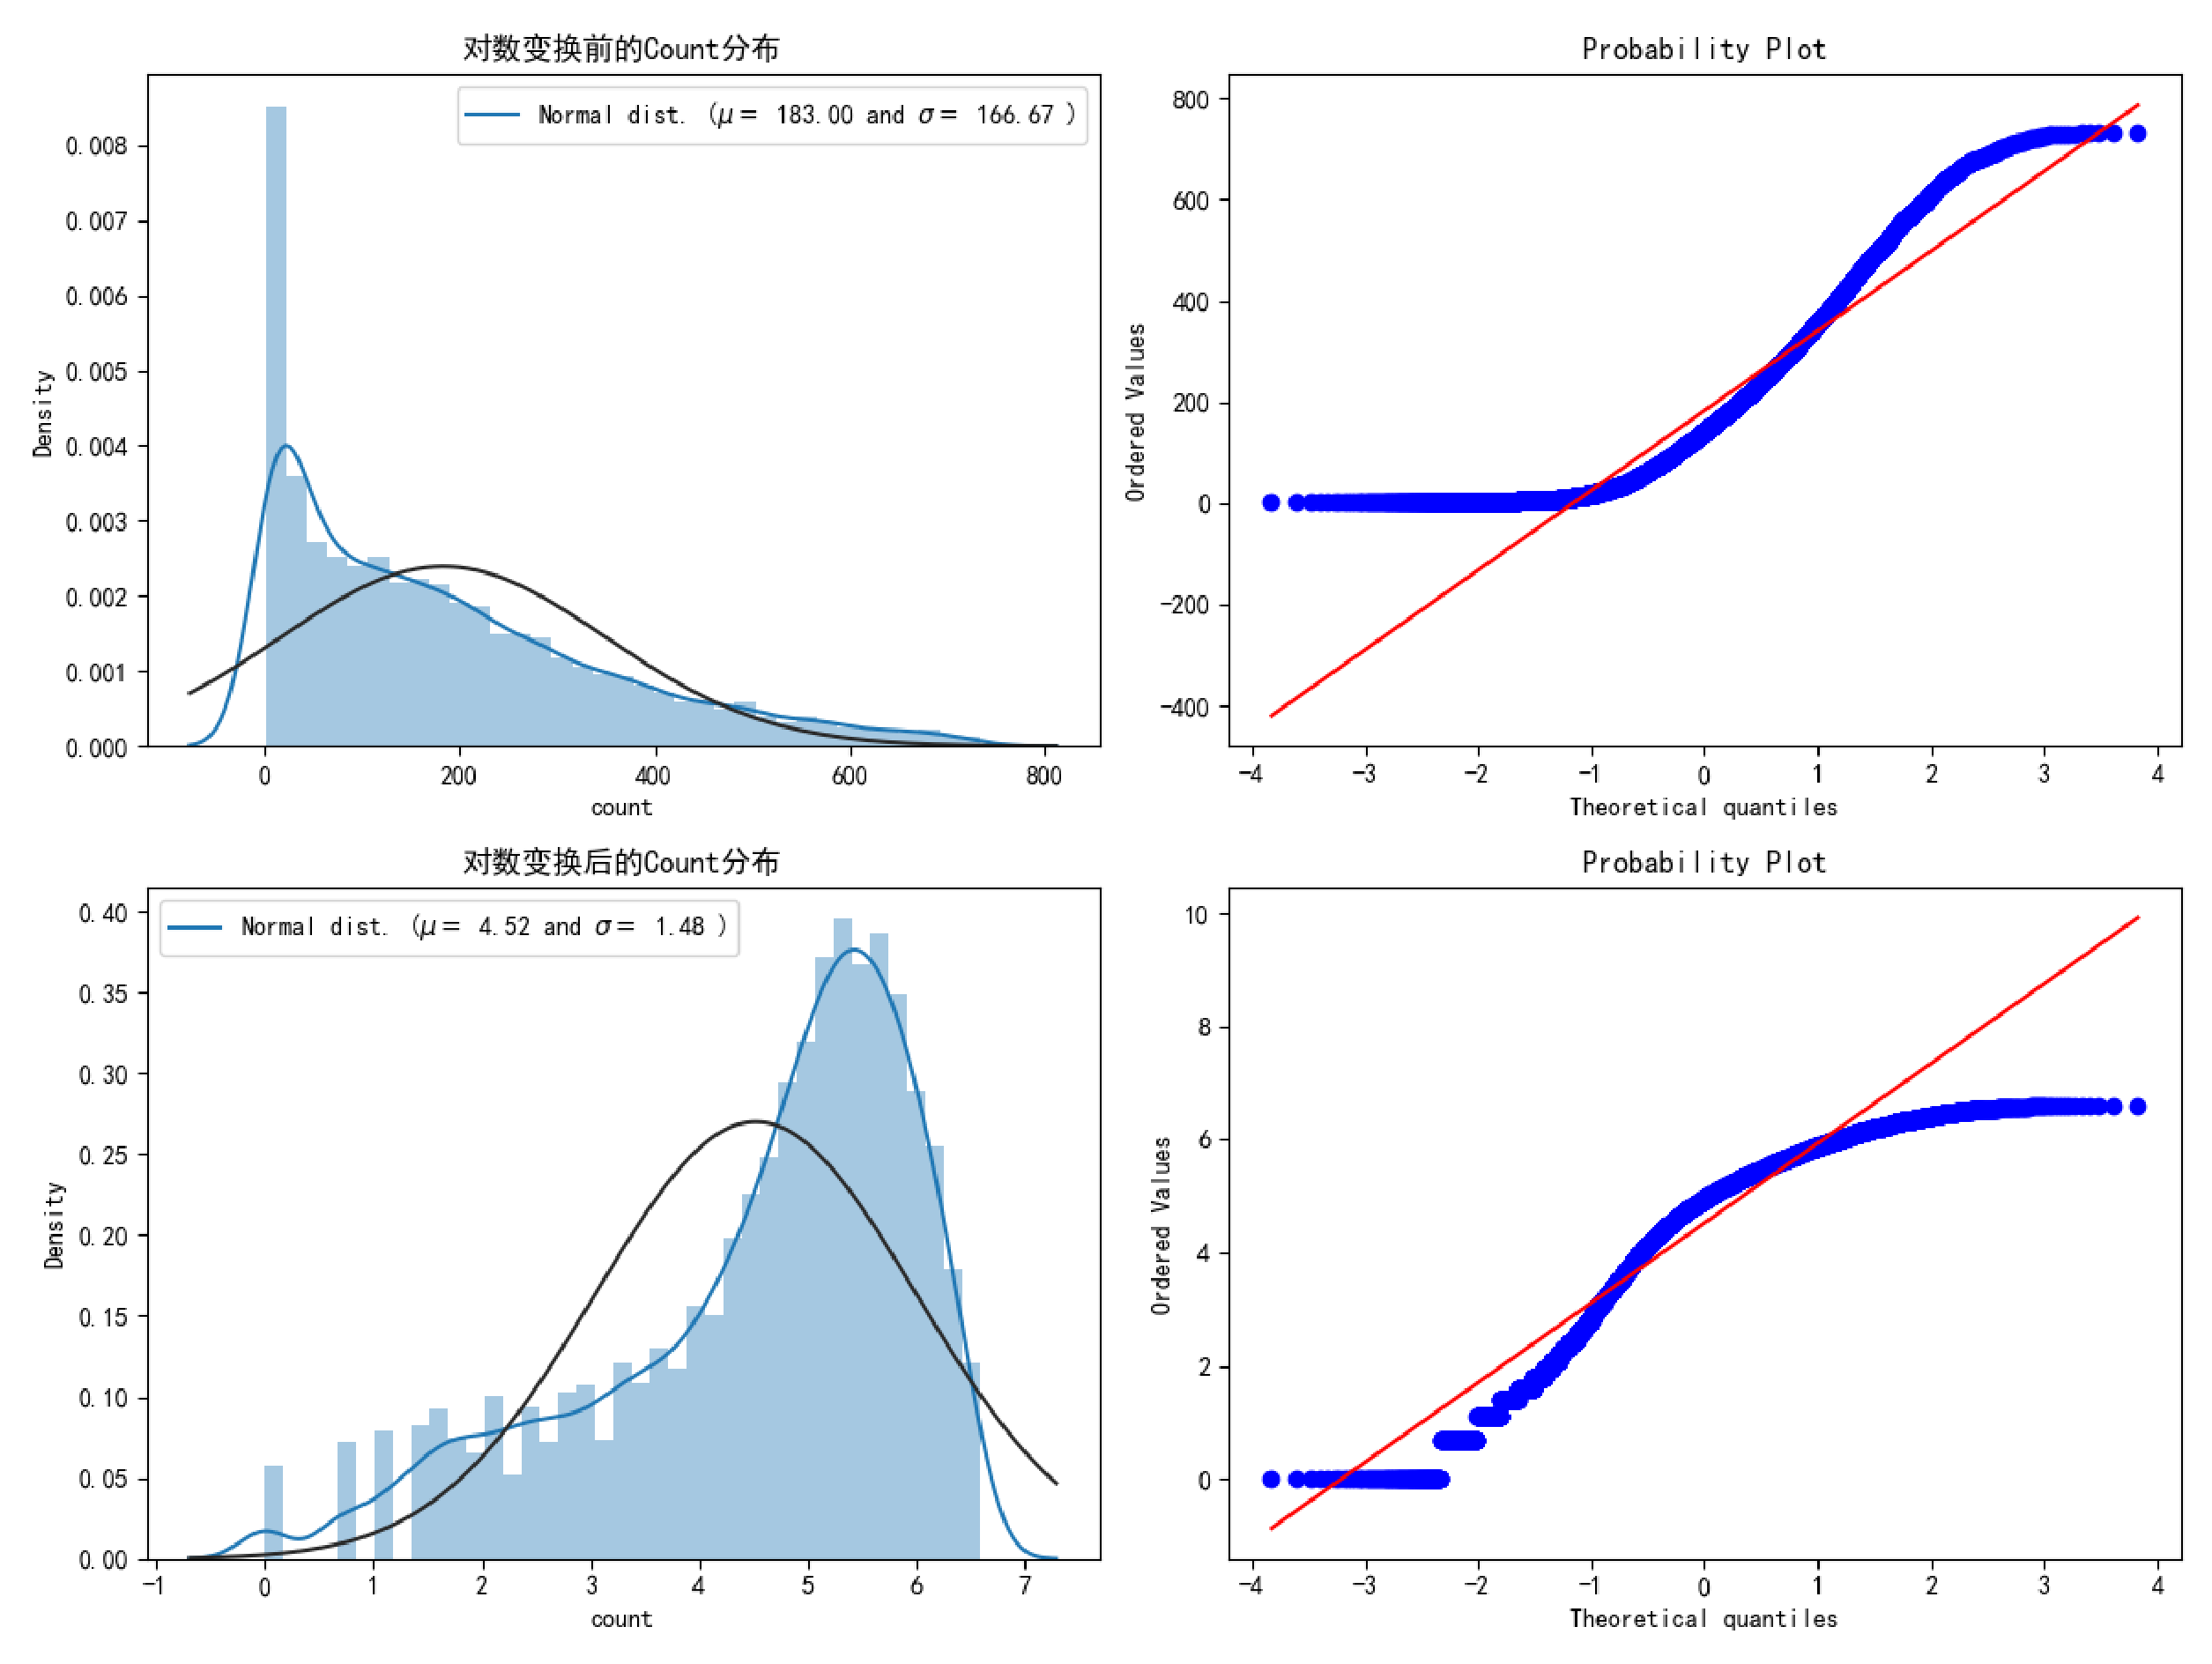
\includegraphics[width=0.8\textwidth,height=0.5\textwidth]{shift.eps}
			\caption{Variable Conversions} \label{framework}
		\end{figure}
	\end{slide}
	%%==========================================================================================
	
	%%==========================================================================================
	%%
	\begin{slide}{Fill In Zero Values}
		The random forest model will be used to fill the zero values in the windspeed feature.
		\begin{figure}[htbp]
			\centering
			\selectcolormodel{rgb}
			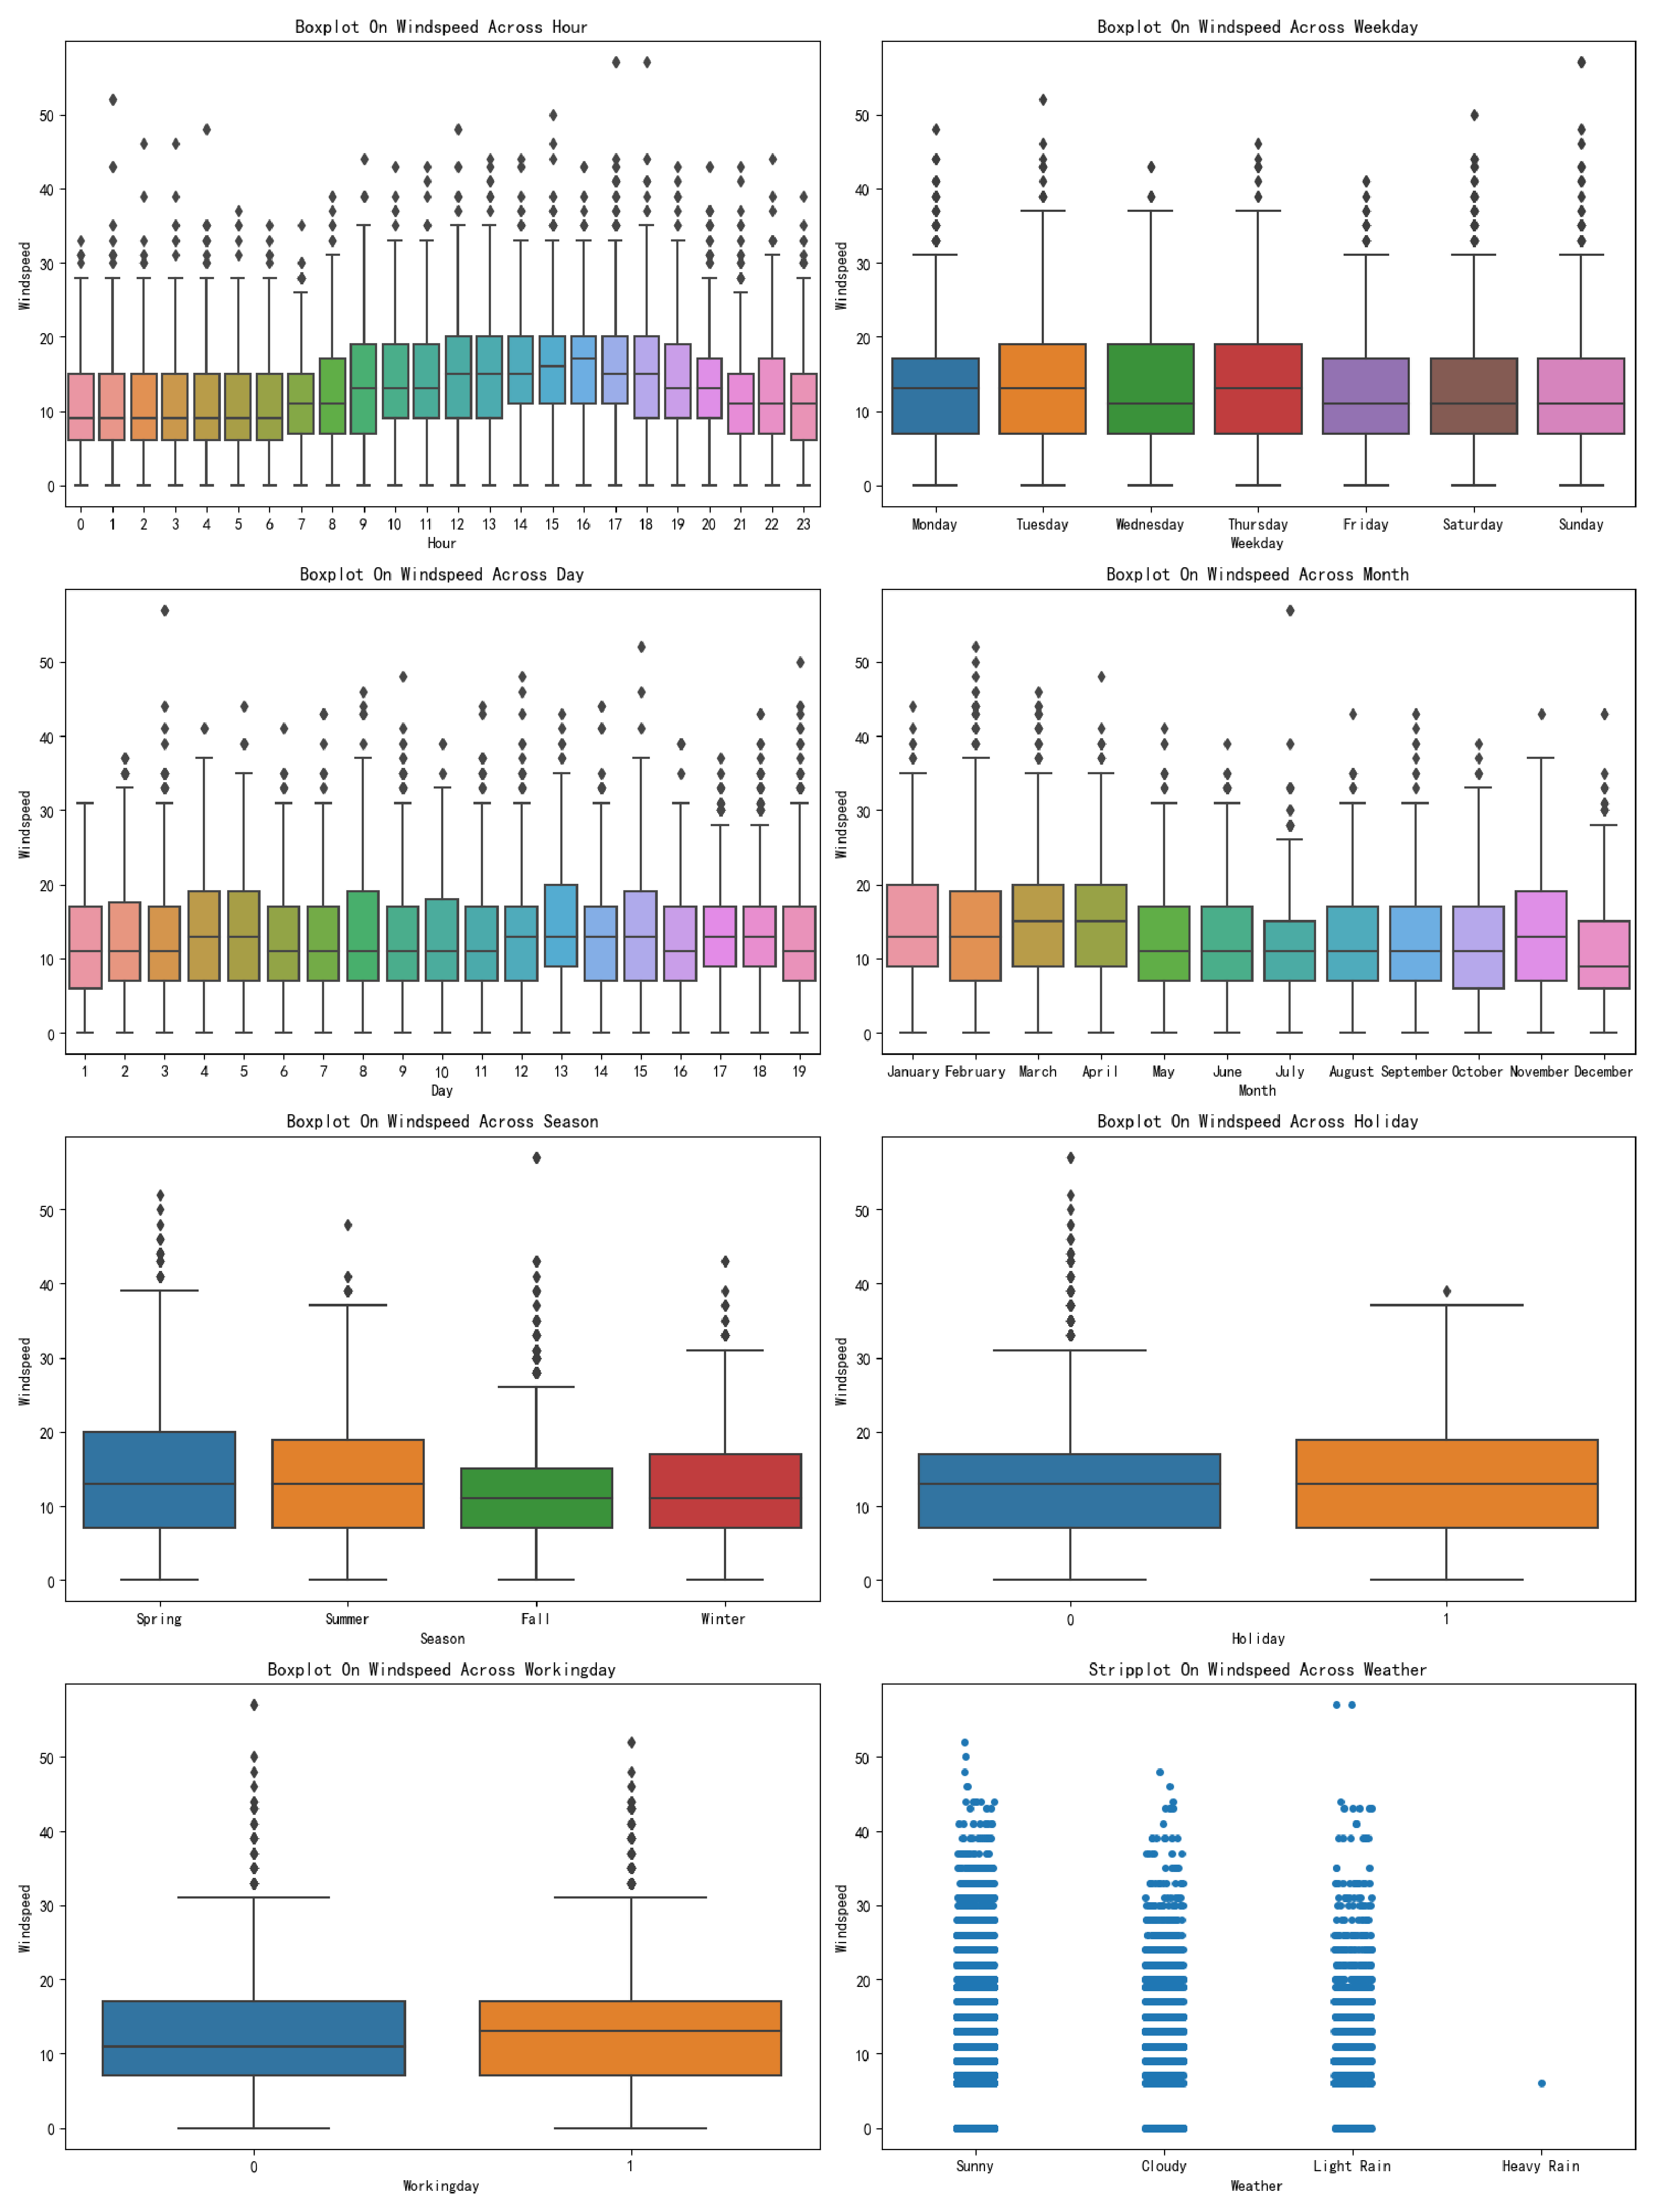
\includegraphics[width=0.8\textwidth,height=0.5\textwidth]{tree.eps}
			\caption{Relationship Between Features and Windspeed} \label{framework}
		\end{figure}
	\end{slide}
	%%==========================================================================================
	
	%%==========================================================================================
	%%
	
	
	\section{Model Solution}
	%%==========================================================================================
	%%
	\begin{slide}{Model Building}
		Summary of RMSLE scores for the 16 models
		\begin{figure}[htbp]
			\centering
			\selectcolormodel{rgb}
			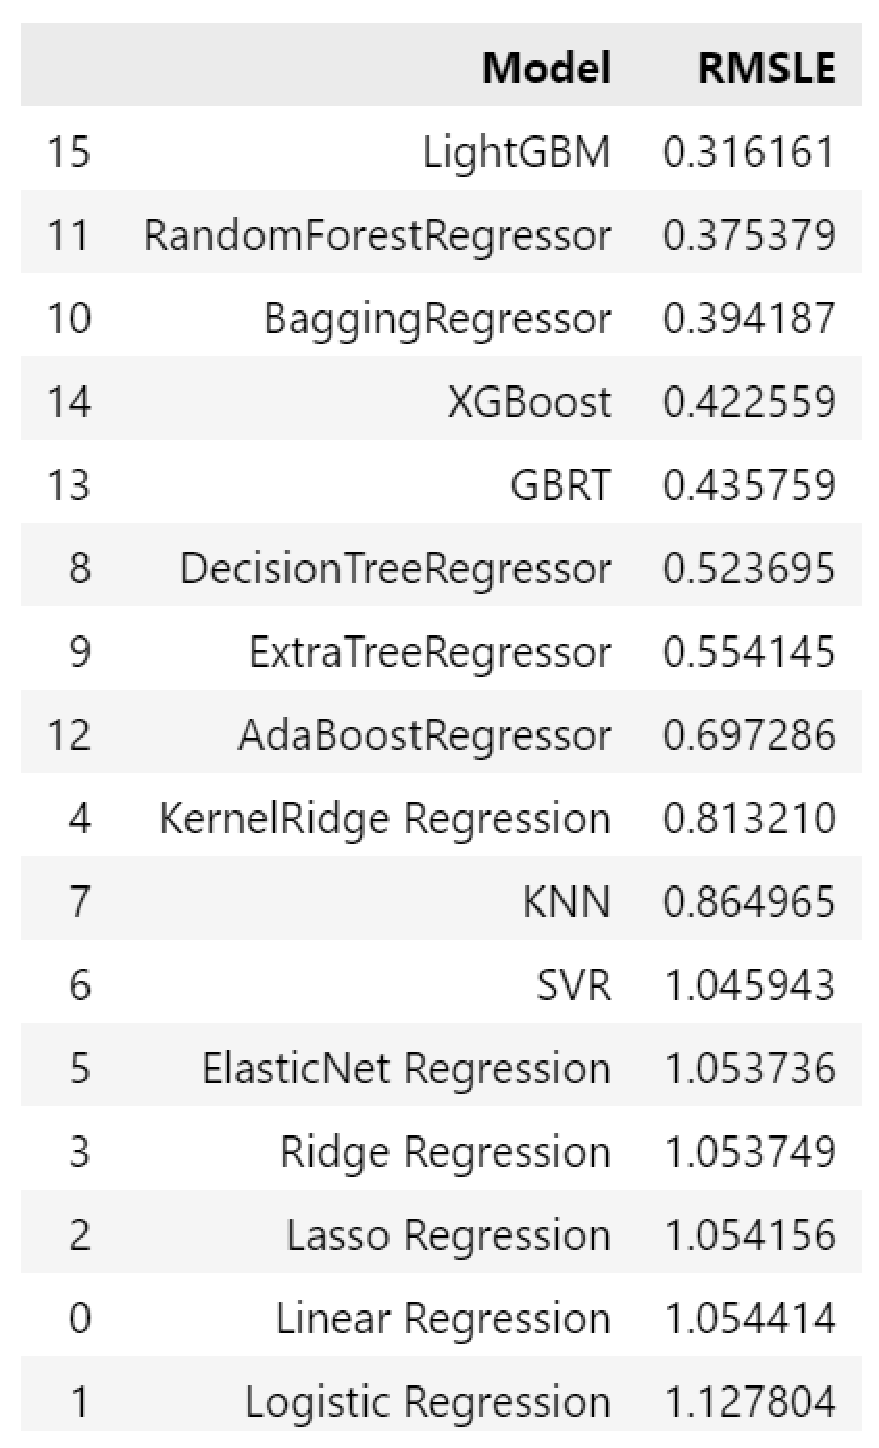
\includegraphics[height=0.5\textwidth]{model.eps}
			\caption{RMSLE Scores} \label{framework}
		\end{figure}
	\end{slide}
	%%==========================================================================================
	%%==========================================================================================
	%%
	\begin{slide}{Model Fusion Stacking}
		\begin{center}
			\centering
			\twotonebox{\rotatebox{90}{}}{\parbox{.86\textwidth}
				{RMSLE For Stacking: 0.3144}}
		\end{center}
	\end{slide}
	
	\begin{slide}{Final prediction result}
		\begin{center}
			\twotonebox{\rotatebox{90}{Result}}{\parbox{.86\textwidth}
				{The best two models Stacking and LightGBM are weighted and the final prediction is saved.
					\\\\ensemble = stacking_pred * 0.60 + lgb_pred * 0.40}}
		\end{center}
	\end{slide}
	
	
\end{document}